%% Calibrated Gating for Adaptive RAG: Knowledge-Based Systems submission
%% Elsevier CAS double-column class.
\documentclass[a4paper,fleqn]{cas-dc}

\usepackage[authoryear]{natbib}
\usepackage{amsmath,amssymb}
\usepackage{booktabs}
\usepackage{array}

\begin{document}
\let\WriteBookmarks\relax

\shorttitle{Calibrated Gating for Adaptive RAG}
\shortauthors{M. A. F. Nayem}

\title[mode=title]{Calibrated Gating for Adaptive RAG: A Conformal Bound on the Decision to Retrieve}

\author[1]{Md Arif Faysal Nayem}[orcid=0009-0003-8576-7197]
\cormark[1]
\ead{mnayem201194@bscse.uiu.ac.bd}
\credit{Conceptualization, Methodology, Software, Formal analysis, Investigation, Data curation, Validation, Visualization, Writing -- original draft, Writing -- review \& editing}
\affiliation[1]{organization={Department of Computer Science and Engineering, United International University},
            addressline={United City, Madani Avenue},
            city={Dhaka},
            postcode={1212},
            country={Bangladesh}}

\cortext[1]{Corresponding author}

\begin{abstract}
Adaptive retrieval-augmented generation (RAG) skips retrieval when a language
model is judged confident enough to answer from parametric memory, trading
accuracy for cost and latency. The component that makes this choice, the
retrieve/skip gate, is safety-critical: a skip taken when the model would
hallucinate sends an unsupported answer to the user. Existing adaptive-RAG gates
(FLARE, Self-RAG, Adaptive-RAG) tune a confidence threshold offline, provide no
formal guarantee on this harmful-skip event, and, as we show, drift across
distributions. We reframe the gate as a risk-controlled
selective-prediction decision under asymmetric cost and apply Conformal Risk
Control (CRC). Given an ignorance score that estimates the probability the model
answers wrongly without retrieval, the gate skips the lowest-scoring queries,
and the threshold is calibrated so the expected harmful-skip rate stays below a
user-chosen tolerance. Because the calibration is conformal, the bound is
finite-sample and distribution-free. The decisive move is what we conformalize:
the gate decision, not the generated answer. On two model families
(Qwen2.5-3B, Phi-3.5-mini) across TriviaQA and PopQA, the realized rate tracks
the target dial almost exactly from a 2\% to a 20\% tolerance. A fixed
threshold calibrated on one distribution overshoots the hallucination budget by
34--58\% on another, whereas per-distribution conformal calibration restores
control. The skip rate auto-scales with model competence (35\% versus 18\% skips
at a fixed tolerance). We characterize when group-conditional (Mondrian)
calibration is needed, only under label shift given features and not proportion
shift, and validate the gate end-to-end with a live retriever as a guaranteed
cost/accuracy dial.
\end{abstract}

\begin{highlights}
\item The retrieve/skip gate in adaptive RAG is recast as risk-controlled selection.
\item Conformal risk control bounds the harmful-skip rate at a user-chosen tolerance.
\item Fixed-threshold gating overshoots the hallucination budget by 34--58\% under shift.
\item The conformal skip rate auto-scales with model competence at a fixed tolerance.
\item Marginal CRC suffices with a calibrated score; Mondrian only for label shift.
\end{highlights}

\begin{keywords}
Adaptive retrieval-augmented generation \sep Conformal risk control \sep
Hallucination mitigation \sep Selective prediction \sep Uncertainty quantification
\end{keywords}

\maketitle

% ======================================================================
\section{Introduction}\label{sec:intro}

Retrieval-augmented generation (RAG) grounds large language models (LLMs) in
external evidence and is now the dominant approach for knowledge-intensive
question answering \citep{lewis2020rag,gao2023ragsurvey}. Retrieval, however, is
not free: it adds latency, monetary cost, and, when irrelevant passages are
returned, can even degrade an answer the model would have produced correctly on
its own. Adaptive RAG therefore makes retrieval optional, invoking it
only when the model appears uncertain \citep{jiang2023flare,asai2024selfrag,
jeong2024adaptiverag}. The component that decides is a binary
retrieve/skip gate.

This gate is a safety-critical decision. When it skips retrieval on a query the
model can in fact answer, it saves cost at no risk. But when it skips on a query
the model would get wrong, the unsupported and often confident answer
reaches the user. We call this event a harmful skip; it is precisely the
hallucination that retrieval was meant to prevent. The two error directions are
not symmetric: an unnecessary retrieval costs a bounded amount of latency, while
a harmful skip costs a hallucination. Treating the gate as an ordinary binary
classifier, optimized for accuracy, ignores this asymmetry.

Existing adaptive-RAG gates fix a confidence threshold (on token probability
\citep{jiang2023flare}, a learned critic token \citep{asai2024selfrag}, or a
query-complexity classifier \citep{jeong2024adaptiverag}) tuned once on a
calibration set. None bounds the harmful-skip rate, and none accounts for the
fact that the threshold's behavior depends on the deployment distribution. We
demonstrate this failure directly: a threshold calibrated on PopQA, applied to
TriviaQA, overshoots a 10\% hallucination budget by 34\% for Qwen2.5-3B and 58\%
for Phi-3.5-mini (Section~\ref{sec:baselines}). The model is more competent on
TriviaQA, so the score distribution shifts, and the fixed threshold silently
becomes unsafe.

\paragraph{Our approach.} We reframe the retrieve/skip gate as a
risk-controlled selective-prediction decision and bring Conformal Risk
Control (CRC) \citep{angelopoulos2024crc} to bear on it. Given an
ignorance score that estimates the probability the model
answers a query wrongly without retrieval, we skip the queries it scores as most
confident. We calibrate the skip threshold on a calibration set so that the
expected harmful-skip rate is bounded by a user-chosen tolerance. Because CRC is
conformal, the bound is finite-sample
and distribution-free: it holds for any score, any model, and any data
distribution, provided calibration and deployment data are exchangeable. The
single move that makes this work is what we conformalize: not the
generated answer, as in prior conformal-RAG and conformal-LLM work
\citep{kumar2023conformalqa,quach2024conformallm}, but the gate decision
itself (Figure~\ref{fig:concept}). The guarantee is placed on the input to
generation (whether to retrieve) rather than its output.

\begin{figure*}[t]
  \centering
  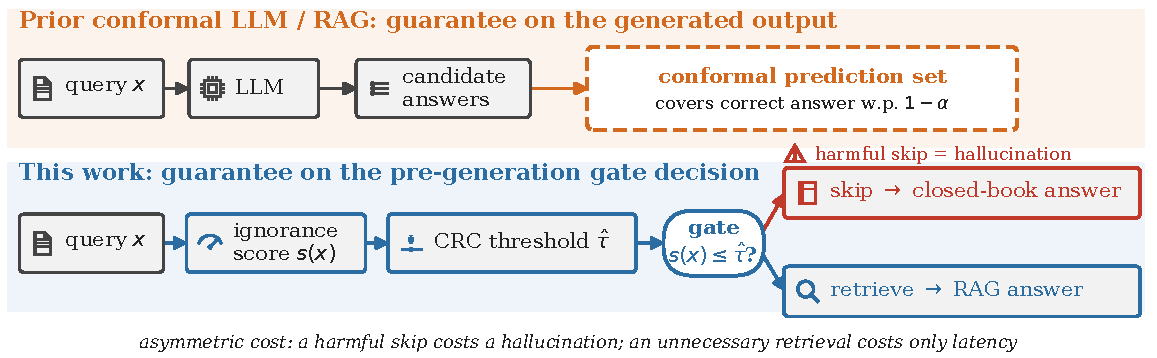
\includegraphics[width=\textwidth]{figs/fig_concept.pdf}
  \caption{What we conformalize. Prior conformal LLM/RAG methods place the
  guarantee on the generated output, wrapping the answer in a prediction set that
  covers the correct answer with high probability (top). We instead place
  the guarantee on the pre-generation gate decision (bottom): an ignorance score
  feeds a CRC-calibrated threshold that chooses skip versus
  retrieve, bounding the harmful-skip rate (a skip on a query the model gets
  wrong, i.e.\ a hallucination) at a user-chosen tolerance. The cost is asymmetric:
  a harmful skip costs a hallucination, whereas an unnecessary retrieval costs
  only latency.}
  \label{fig:concept}
\end{figure*}

\paragraph{Contributions.}
\begin{enumerate}[(1)]
\item We formalize the retrieve/skip gate as a risk-controlled
selective-prediction decision under asymmetric cost, identifying the gate
decision (not the generated answer) as the right object to conformalize, and
derive a CRC-calibrated gate that bounds the expected harmful-skip rate at any
user-chosen tolerance (Section~\ref{sec:method}).
\item We show on real LLM behavior that the realized harmful-skip rate tracks the
target dial almost exactly from a 2\% to a 20\% tolerance, whereas the prevailing
fixed-threshold practice overshoots the hallucination budget by 34--58\% under
distribution shift, which per-distribution conformal calibration corrects
(Sections~\ref{sec:dial}--\ref{sec:baselines}).
\item We show the conformal skip rate auto-scales with model competence at a fixed
tolerance, turning skip rate into an emergent measure of what the model knows, and
that every result replicates across two model families
(Section~\ref{sec:efficiency}).
\item We characterize when group-conditional (Mondrian) calibration is
needed, only under label-shift-given-features and not proportion shift, and
validate the gate end-to-end with a live retriever as a guaranteed cost/accuracy
dial (Sections~\ref{sec:mondrian}--\ref{sec:e2e}).
\end{enumerate}

% ======================================================================
\section{Related work}\label{sec:related}

\subsection{Retrieval-Augmented Generation and adaptive retrieval}

Retrieval-Augmented Generation \citep{lewis2020rag} grounds LLM inference in
external evidence, substantially improving factual accuracy on knowledge-intensive
tasks \citep{gao2023ragsurvey,karpukhin2020dpr}. Unconditional retrieval,
however, adds latency and cost, and context that is irrelevant to a query the
model already knows can degrade accuracy \citep{yan2024crag}. This motivates
adaptive retrieval strategies.

FLARE \citep{jiang2023flare} monitors generation-time token probability and
retrieves whenever it falls below a hand-tuned threshold. Self-RAG
\citep{asai2024selfrag} trains the LLM itself to emit a special reflection token
(\texttt{[Retrieve]} / \texttt{[No Retrieve]}), framing the gate as a generation
task. Adaptive-RAG \citep{jeong2024adaptiverag} trains a separate complexity
classifier to route each query to no-retrieval, single-step, or multi-step
retrieval. DRAGIN \citep{su2024dragin} operates at the token level, triggering
retrieval when the entropy of the next-token distribution exceeds a threshold.
Corrective RAG \citep{yan2024crag} adds a lightweight retrieval evaluator that
judges retrieved document quality and, when documents are deemed unreliable,
escalates to a web search, introducing a form of retrieval confidence without
a formal guarantee.

All of these methods fix or learn a decision boundary on a training or
calibration distribution, without providing any guarantee on the harmful-skip
error rate, and without re-calibrating to the deployment distribution. We
demonstrate in Section~\ref{sec:baselines} that this failure is measurable and
systematic: a threshold calibrated on one dataset overshoots the hallucination
budget by 34--58\% on another. Our contribution is orthogonal to the choice of
uncertainty signal: FLARE's token probability, Self-RAG's reflect score, or
DRAGIN's entropy can all serve as features in our ignorance score, after which
CRC supplies the missing finite-sample guarantee.

\subsection{Conformal prediction}

Conformal prediction \citep{vovk2005algorithmic} constructs prediction sets that
contain the true label with user-specified probability under exchangeability,
with no assumptions on the data distribution. \citet{angelopoulos2023gentle}
provide a modern tutorial. Conformal Risk Control (CRC)
\citep{angelopoulos2024crc} generalizes coverage to any monotone, bounded loss
$L$, bounding $\mathbb E[L]\le\alpha$ via a one-dimensional threshold search, the
formulation we use for harmful-skip control. Risk-Controlling Prediction Sets
\citep{bates2021riskcontrolling} provide a training-conditional (PAC-style)
variant; the expected-value CRC guarantee we use is weaker but requires no
learning. Group-conditional (Mondrian) conformal prediction
\citep{vovk2012conditional} delivers per-group validity; covariate-shift
corrections \citep{tibshirani2019covariate} handle distribution mismatches. We
use these to characterize precisely when marginal CRC is insufficient
(Section~\ref{sec:mondrian}).

\subsection{Conformal prediction for LLMs and RAG}

\textbf{Conformalizing the answer.} The majority of conformal-LLM work controls a
property of the model's output. \citet{kumar2023conformalqa} construct
prediction sets for multiple-choice QA that cover the correct option with high
probability. \citet{quach2024conformallm} develop conformal language modeling,
stopping sequential generation once a coverage guarantee is satisfied. TRAQ
\citep{li2024traq} is the most directly related prior work: it applies conformal
prediction end-to-end to RAG at both retriever and generator stages, guaranteeing
with high probability that the prediction set contains a semantically correct
answer. \citet{ren2023knowno} apply conformal prediction to LLM-based robot
planning. \citet{xiong2024llmuncertainty} show that eliciting calibrated
confidence from an LLM is non-trivial and model-dependent.

\textbf{Conformalizing abstention.} Closest in spirit to our work is
\citet{abbasiyadkori2024conformalabstention}, who apply conformal abstention at
the generation level: the model outputs ``I don't know'' when its
self-consistency score is below a CRC-calibrated threshold, bounding the
hallucination rate on non-abstained queries. Our gate operates at the
retrieval level, deciding whether to retrieve before any generation
occurs, and its asymmetric cost formulation (a harmful skip costs a
hallucination; an unnecessary retrieval costs only latency) is specific to the
RAG setting.

\textbf{The critical distinction.} All prior conformal-LLM work controls a
property of the model's output or post-generation decision; we control the
pre-generation input decision: whether to retrieve. This is a structurally
distinct guarantee (applied to the binary gate rather than the answer) that,
to our knowledge, has not previously been addressed.

\subsection{Uncertainty estimation for LLMs}

Informative uncertainty signals are available across multiple modalities.
Token log-probability is a strong scalar baseline and emerges as genuine
self-knowledge in capable LLMs \citep{kadavath2022know}; calibration of
neural confidences under distribution shift is a known challenge
\citep{guo2017calibration,xiong2024llmuncertainty}. Self-consistency
\citep{wang2023selfconsistency} aggregates multiple samples to reduce surface-form
variability. Semantic entropy \citep{kuhn2023semantic} estimates uncertainty at
the meaning level, avoiding spurious variance from paraphrase;
\citet{farquhar2024detecting} demonstrate this is effective for hallucination
detection in real LLMs. Black-box consistency checking via SelfCheckGPT
\citep{manakul2023selfcheckgpt} requires no access to model logits.
\citet{ji2023hallucination} survey LLM hallucination broadly. We use a
multivariate logistic model over these signals (Section~\ref{sec:score}); a key
empirical finding is that signal granularity (density of distinct score
values) matters more than discriminative power for CRC efficiency, a design
principle absent from prior uncertainty-estimation work.

\subsection{Selective prediction}

Selective prediction \citep{geifman2017selective} frames a coverage/accuracy
trade-off for an abstaining classifier. We apply this lens to the retrieval
decision: the model ``abstains'' from answering without retrieval when uncertain,
handing off to the retriever as its safe fallback. Unlike classical selective
prediction, our cost structure is asymmetric: the cost of a harmful abstention
(skipping retrieval when the model is wrong) far exceeds the cost of unnecessary
retrieval (latency). This asymmetry motivates CRC over standard
coverage-maximizing selective prediction \citep{geifman2017selective}.

% ======================================================================
\section{Method}\label{sec:method}

\subsection{The gate as risk-controlled selective prediction}\label{sec:formal}

Let $x$ be a query, $M$ an LLM, and $R$ a retrieval pipeline. A gate
$d(x)\in\{\textsc{skip},\textsc{retrieve}\}$ decides whether $M$ answers $x$
from parametric memory (\textsc{skip}) or with retrieved evidence
(\textsc{retrieve}). Let $w(x)$ be the indicator that $M$ answers $x$ wrongly
without retrieval. The safety-critical event is the harmful skip,
\begin{equation}
h(x)\;=\;\mathbf 1[d(x)=\textsc{skip}]\cdot w(x),
\end{equation}
a skip taken on a query the model gets wrong, an avoidable hallucination. The
cost structure is asymmetric: an unnecessary retrieval ($d=\textsc{retrieve}$,
$w=0$) costs bounded latency, while a harmful skip costs an ungrounded answer.
We therefore do not seek the accuracy-optimal gate; we seek the gate that
minimizes retrieval subject to a cap on harmful skips:
\begin{equation}\label{eq:objective}
\min_{d}\ \mathbb E\big[\mathbf 1[d(x)=\textsc{retrieve}]\big]
\quad\text{s.t.}\quad \mathbb E[h(x)]\le\alpha,
\end{equation}
for a user-chosen tolerance $\alpha\in(0,1)$. This is selective prediction
\citep{geifman2017selective} applied to retrieval, with the abstention direction
(here, \textsc{retrieve}) treated as the safe fallback.

\subsection{Ignorance score}\label{sec:score}

We summarize the model's per-query ignorance with a scalar $s(x)\in[0,1]$,
higher meaning more likely wrong without retrieval. From $k=8$ closed-book
samples we extract four features: negative mean token log-probability of the
greedy answer \citep{kadavath2022know}; semantic entropy over
normalized-answer clusters \citep{kuhn2023semantic}; one minus self-consistency
(the fraction of samples agreeing with the greedy answer)
\citep{wang2023selfconsistency}; and answer length. A multivariate logistic
\textsc{IgnoranceModel} maps these to $\hat P(w=1\mid x)$, which is $s(x)$.

Two empirical facts shape this design (Sections~\ref{sec:dial}--\ref{sec:baselines}).
First, the individual signals have nearly identical discriminative power
(AUROC for predicting $w$ ranges $0.85$--$0.89$; Table~\ref{tab:auroc}), so the
choice among them is not about information content. Second, what matters
for CRC is granularity: a discrete score with few distinct values cannot
place a threshold that spends the budget precisely. Discrete semantic entropy
from $k=8$ samples is too coarse, spending only $\approx3.7\%$ of a $10\%$
budget, whereas the continuous log-probability (and the logistic score that
inherits its granularity) uses the budget fully at the same AUROC. We therefore
use the continuous multivariate score throughout.

\subsection{Conformal Risk Control of the gate}\label{sec:crc}

The gate is a threshold rule, $d(x)=\textsc{skip}\iff s(x)\le\tau$. Smaller
$\tau$ skips fewer (only the most confident) queries, so the harmful-skip rate
is monotone non-decreasing in $\tau$. Given a calibration set
$\{(s_i,w_i)\}_{i=1}^{n}$ of scored, graded queries, we set
\begin{equation}\label{eq:crc}
\hat\tau \;=\; \max\Big\{\tau:\ \frac{1+\sum_{i=1}^{n}\mathbf 1[s_i\le\tau]\,w_i}{n+1}\ \le\ \alpha\Big\}.
\end{equation}
Under exchangeability of calibration and test data, Conformal Risk Control
\citep{angelopoulos2024crc} guarantees
\begin{equation}
\mathbb E[h(x_{\text{test}})] \;\le\; \alpha,
\end{equation}
where the expectation is over the draw of calibration and test points. The
$+1$ in the numerator and $n+1$ in the denominator are the finite-sample
correction; they make the bound hold exactly at any $n$, at the cost of slight
conservatism that vanishes as $n\to\infty$. This is a correctness
property, preventing the small-sample overshoot that an uncorrected empirical
quantile incurs, rather than the efficiency headline. Since the harmful-skip rate
is monotone non-decreasing in $\tau$, $\hat\tau$ is the largest threshold
satisfying the constraint in \eqref{eq:objective}, hence it minimizes retrieval
frequency subject to the guarantee.

Exchangeability holds when calibration and deployment queries are drawn i.i.d.\
from the same distribution, the standard assumption for split-conformal procedures.
When a known covariate shift is present, the weighted extension of
\citet{tibshirani2019covariate} restores validity at the cost of a
density-ratio estimate over the shift covariates.

\subsection{Baselines}\label{sec:baselinesdef}

We compare the CRC gate against: \textbf{never-retrieve} and
\textbf{always-retrieve} (the trivial endpoints); \textbf{tuned-threshold}, the
empirical $\alpha$-quantile of $\{s_i:w_i=1\}$ with no finite-sample correction;
\textbf{fixed-threshold}, the same threshold calibrated on one distribution and
deployed on another without re-calibration, representing any gate that does not
adapt its threshold at deployment time; and
\textbf{group-conformal (Mondrian)}, one CRC threshold per novelty bucket so
that $\mathbb E[h\mid\text{bucket}]\le\alpha$ within each bucket.

\subsection{When is group-conditional control needed?}\label{sec:mondrian-method}

Marginal CRC \eqref{eq:crc} bounds the overall expected harm. Under
distribution shift one might fear it fails on the worst sub-population. We show
(Section~\ref{sec:mondrian}) that when the score is approximately conditionally
calibrated ($s(x)\approx P(w=1\mid x)$, which a multivariate logistic score on
informative features achieves), marginal CRC already yields near-per-bucket
control, because the score captures the very feature axes along which the
distribution shifts. Group-conditioning becomes necessary only under
label-shift-given-features: when two groups share feature values but
differ in $P(w\mid\text{features})$, so the score cannot tell them apart. That
case requires knowing the shift axis in advance and pre-declaring buckets.

% ======================================================================
\section{Experimental setup}\label{sec:setup}

\paragraph{Models and data.} We use two instruction-tuned LLMs from different
families, Qwen2.5-3B-Instruct \citep{qwen2025technical} and Phi-3.5-mini-instruct
\citep{abdin2024phi3}, in fp16 on a single GPU. We evaluate on two open-domain
QA datasets with contrasting difficulty: PopQA \citep{mallen2023popqa} (test
split, popularity-stratified 1000 questions; long-tail-heavy) and TriviaQA
\citep{joshi2017triviaqa} (\texttt{rc.nocontext} validation, 1000 questions;
more head entities). Closed-book accuracy is 0.126/0.365 (Qwen) and 0.140/0.434
(Phi) on PopQA/TriviaQA, giving a wide competence gap to test adaptive
behavior.

\paragraph{Protocol.} For each query we draw $k=8$ samples (one greedy, seven
temperature-sampled), grade correctness by exact match against gold answer
aliases, and extract the four ignorance features. We fit the
\textsc{IgnoranceModel} on a held-out fold and report all gate metrics over $10$
random calibration/test splits ($n_{\text{cal}}\approx333$, one-third of the
1000-question pool; CRC remains valid at any $n$ by construction, as the
finite-sample correction in \eqref{eq:crc} absorbs small-$n$ variance), as
mean$\pm$std. AUROC values are pooled across datasets.

\paragraph{End-to-end retriever.} For the downstream evaluation
(Section~\ref{sec:e2e}) we attach a live retriever (MediaWiki subject-page
search; context-hit 100\%, answer-in-context $\approx$84\% on PopQA). A skip
yields the closed-book answer; a retrieve yields the RAG answer over the
retrieved context.

\paragraph{Synthetic shift probe.} To exhibit the regime where Mondrian is
required (Section~\ref{sec:mondrian}) we use a controlled generator with a known
$P(w\mid x)$ and two novelty buckets (popular, $p_{\text{know}}=0.85$;
long-tail, $p_{\text{know}}=0.25$), calibrating on a 20\% long-tail mixture and
deploying on a 70\% long-tail mixture (200 draws).

% ======================================================================
\section{Results}\label{sec:results}

\subsection{The safety guarantee holds and is not conservative}\label{sec:dial}

Figure~\ref{fig:dial} and Table~\ref{tab:dial} report the realized harmful-skip
rate as the target $\alpha$ is swept from $0.02$ to $0.20$. On both model
families the realized rate tracks the dial almost exactly: for example, for
Qwen2.5-3B (pooled), $\alpha=0.02\to0.05\to0.10\to0.15\to0.20$ yields realized
$0.019\to0.049\to0.098\to0.149\to0.199$, and Phi-3.5-mini matches to within a
point at every setting. The guarantee is therefore not merely satisfied but
tight: the gate spends the budget rather than hiding behind needless
retrieval. Retrieval frequency falls monotonically as $\alpha$ rises
(Figure~\ref{fig:dial}b), so $\alpha$ acts as a single interpretable cost dial.

\begin{figure*}[t]
  \centering
  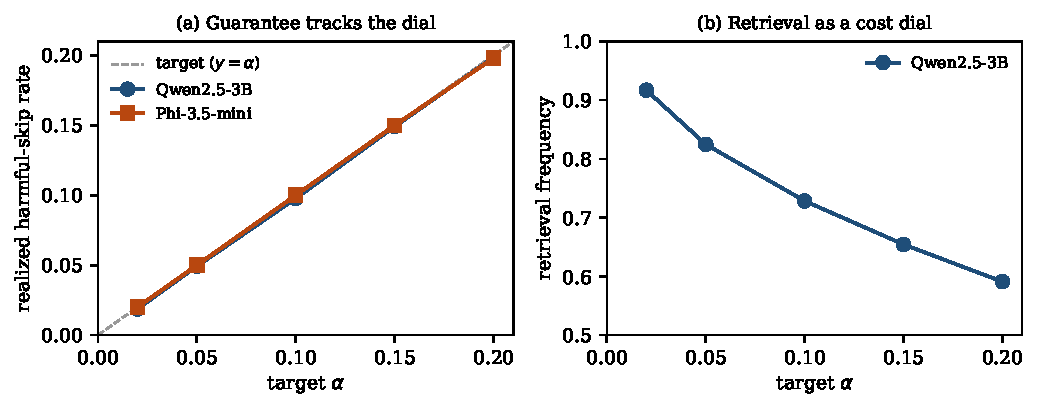
\includegraphics[width=\textwidth]{figs/fig1_coverage.pdf}
  \caption{The conformal guarantee on real LLM behavior. (a) Realized
  harmful-skip rate vs.\ target $\alpha$ for both model families; the dashed line
  is $y=\alpha$. (b) Retrieval frequency falls monotonically as the budget
  loosens, so $\alpha$ is an interpretable cost dial. Mean over 10
  calibration/test splits.}
  \label{fig:dial}
\end{figure*}

\begin{table*}[width=\textwidth,cols=6,pos=h]
\caption{Coverage dial (Qwen2.5-3B, pooled). Realized harmful-skip rate tracks
target $\alpha$; retrieval trades off monotonically.}\label{tab:dial}
\begin{tabular*}{\tblwidth}{@{} lRRRRR @{}}
\toprule
target $\alpha$ & 0.02 & 0.05 & 0.10 & 0.15 & 0.20\\
\midrule
realized harm & 0.019 & 0.049 & 0.098 & 0.149 & 0.199\\
retrieval freq & 0.917 & 0.825 & 0.728 & 0.654 & 0.591\\
\bottomrule
\end{tabular*}
\end{table*}

\begin{table}[width=.9\linewidth,cols=3,pos=h]
\caption{AUROC of ignorance signals for predicting wrongness (pooled,
TriviaQA$+$PopQA). Discriminative power is near-identical; the operative
difference is score granularity, not information
(Section~\ref{sec:score}). Dashes indicate signals not computed for
Phi-3.5-mini: the $k=8$ sampling budget for semantic entropy and
self-consistency was allocated to Qwen for the primary granularity
analysis; accordingly the \textsc{IgnoranceModel} for Phi-3.5-mini uses
neg.\ log-prob and answer length only, consistent with its AUROC of
$0.888$.}\label{tab:auroc}
\begin{tabular*}{\tblwidth}{@{} LRR @{}}
\toprule
signal & Qwen2.5-3B & Phi-3.5-mini\\
\midrule
neg.\ mean log-prob & 0.881 & 0.888\\
semantic entropy & 0.861 & n/a\\
$1-$self-consistency & 0.854 & n/a\\
\bottomrule
\end{tabular*}
\end{table}

\subsection{Fixed-threshold gating is unsafe under distribution shift}\label{sec:baselines}

The central practical claim is that the prevailing fixed-threshold practice
silently breaks under distribution change. Table~\ref{tab:baselines} fixes
$\alpha=0.10$ and compares gates. A threshold calibrated on PopQA and deployed on
TriviaQA realizes harm $0.134$, a 34\% overshoot of the budget in the dangerous
direction; the reverse calibration is over-conservative (harm $0.069$, wasting
retrieval). Per-distribution conformal calibration hits the target on each
distribution ($0.098$ on TriviaQA, $0.097$ on PopQA). The same failure is
worse on Phi-3.5-mini: the PopQA$\to$TriviaQA threshold overshoots by
58\%. The reason is exactly the competence gap: the score distribution shifts
between datasets, so a threshold frozen on one is mis-calibrated on the other.
Conformal recalibration, being distribution-free, adapts automatically.

\begin{table*}[width=\textwidth,cols=4,pos=h]
\caption{What conformal gating buys ($\alpha=0.10$). A fixed threshold (calibrated
once, deployed without re-calibration to the new domain) drifts with the
deployment distribution; only per-distribution conformal calibration hits the
target with a guarantee. The fixed-threshold rows model any deployment that does
not adapt its threshold at the target domain. Harm $=$ realized harmful-skip rate.}
\label{tab:baselines}
\begin{tabular*}{\tblwidth}{@{} LRRR @{}}
\toprule
gate & TriviaQA & PopQA & controlled?\\
\midrule
never-retrieve & 0.635 & 0.874 & no (catastrophic)\\
always-retrieve & 0.000 & 0.000 & safe, retr.\,$=1$\\
fixed thr.\ (PopQA$\to$Triv.) & \textbf{0.134} & n/a & \textbf{no, $+$34\%}\\
fixed thr.\ (Triv.$\to$PopQA) & n/a & 0.069 & no, over-cons.\\
\textbf{conformal (per-dist.)} & \textbf{0.098} & \textbf{0.097} & \textbf{yes}\\
\bottomrule
\end{tabular*}
\end{table*}

\subsection{Adaptive efficiency and generality}\label{sec:efficiency}

At a fixed budget $\alpha=0.10$, the gate skips more on the dataset the model
knows better, with no re-tuning (Table~\ref{tab:efficiency}). Qwen2.5-3B skips
35\% of TriviaQA but only 18\% of PopQA; Phi-3.5-mini skips 42\% vs 20\%. The
skip rate is thus an emergent measure of model competence: the more the
model knows, the more retrieval the gate safely declines, all while holding the
same hallucination guarantee. Every core result (the coverage dial, the
fixed-threshold failure, and adaptive skipping) replicates across both model
families, indicating the findings are not model-specific.

\begin{table*}[width=\textwidth,cols=5,pos=h]
\caption{Adaptive efficiency and cross-family generality ($\alpha=0.10$). Skip
rate scales with closed-book competence at a fixed hallucination guarantee.}
\label{tab:efficiency}
\begin{tabular*}{\tblwidth}{@{} LRRRR @{}}
\toprule
& \multicolumn{2}{c}{Qwen2.5-3B} & \multicolumn{2}{c}{Phi-3.5-mini}\\
\cmidrule(lr){2-3}\cmidrule(lr){4-5}
dataset & acc & skip & acc & skip\\
\midrule
TriviaQA & 0.365 & 35\% & 0.434 & 42\%\\
PopQA & 0.126 & 18\% & 0.140 & 20\%\\
\bottomrule
\end{tabular*}
\end{table*}

\subsection{When is group-conditional control needed?}\label{sec:mondrian}

\begin{figure*}[tb]
  \centering
  \begin{minipage}[t]{0.49\textwidth}
    \centering
    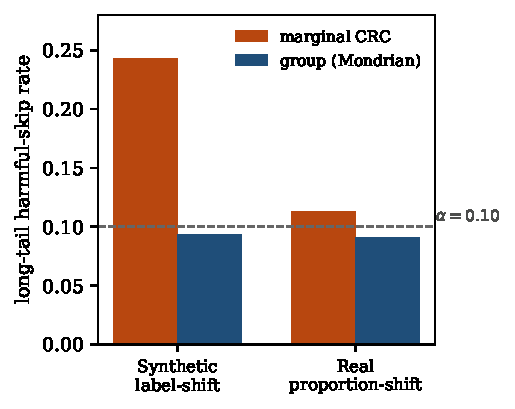
\includegraphics[width=\linewidth]{figs/fig3_mondrian.pdf}
  \end{minipage}\hfill
  \begin{minipage}[t]{0.49\textwidth}
    \centering
    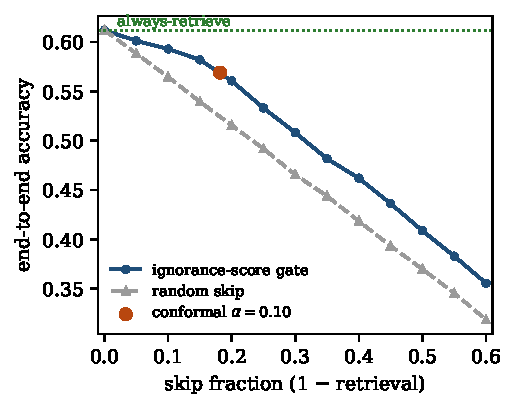
\includegraphics[width=\linewidth]{figs/fig4_endtoend.pdf}
  \end{minipage}
  \caption{(a) When group-conditioning is needed ($\alpha=0.10$, long-tail harm).
  Under synthetic label-shift, marginal CRC violates the budget and Mondrian is
  required; under real proportion-shift, a conditionally-calibrated score keeps
  marginal CRC near $\alpha$ without grouping. (b) End-to-end accuracy vs.\ skip
  fraction on PopQA with a live retriever. The ignorance-score gate beats random
  skipping at every budget; the always-retrieve line and the conformal
  $\alpha=0.10$ operating point are marked. The gate is a guaranteed cost/accuracy
  dial.}
  \label{fig:results}
\end{figure*}

Figure~\ref{fig:results}(a) contrasts two shift regimes at $\alpha=0.10$, reporting
harm on the long-tail sub-population. Under a synthetic label-shift
(calibration 20\% $\to$ deployment 70\% long-tail, with bucket-dependent
$P(w\mid x)$), marginal CRC blows the budget on the long tail (harm $0.243$,
$2.4\times\alpha$) while group-conditional CRC restores control (harm $0.094$),
at modestly higher retrieval. This is the textbook case for Mondrian. On
real data, however, the same 20\%$\to$70\% long-tail proportion shift
leaves marginal CRC barely over budget (long-tail harm $0.113$ vs group
$0.091$), and across four real shift configurations marginal CRC never violates
$\alpha$ by more than $0.013$. The reason is that the multivariate ignorance
score is approximately conditionally calibrated, so proportion shifts in
buckets it can already distinguish do not break marginal control. The design
guidance is therefore precise: use marginal CRC with a good score; reserve
Mondrian for known label-shift-given-features.

\subsection{End-to-end validation with a live retriever}\label{sec:e2e}

Attaching a real retriever (Section~\ref{sec:setup}) lets us measure final
answer accuracy against retrieval cost on PopQA (Figure~\ref{fig:results}(b)). Three
reference points frame the result: never-retrieve $0.126$, always-retrieve
$0.612$, and an oracle gate $0.628$ at $0.874$ retrieval. The ignorance-score
gate dominates uninformed (random) skipping at every retrieval budget,
confirming the score is end-to-end meaningful, and the oracle's edge over
always-retrieve shows there is real headroom for gating.

We are deliberately careful about what this does and does not show. On PopQA the
retrieval fix-rate (0.57, the chance retrieval rescues a wrong closed-book
answer) far exceeds the poison-rate (0.13, the chance it spoils a correct one),
and only 12.6\% of questions are answerable closed-book. Retrieval is thus
beneficial even on the queries the gate would skip, so selective retrieval here
cannot beat full RAG on accuracy; the conformal gate is a
guaranteed cost/accuracy dial (e.g.\ cut 18\% of retrievals for $-4.3$
accuracy points, with harmful skips bounded by $\alpha$), not an accuracy win.
The accuracy-positive regime requires a workload with a genuine
closed-book-answerable head, where retrieval is wasteful or harmful.
Analytically, the gate beats full RAG exactly when the poison avoided on
skipped-known queries exceeds the fixes lost on skipped-unknown queries, a
condition our PopQA numbers do not meet. We report the downstream result honestly as cost control with
demonstrated headroom, not as an accuracy improvement.

% ======================================================================
\section{Discussion}\label{sec:discussion}

\paragraph{A dial, not just a gate.} FLARE and Self-RAG expose one operating
point per threshold; the conformal gate exposes a controlled frontier
indexed by an interpretable risk level $\alpha$. An operator who can state an
acceptable hallucination-from-skipping rate gets the cheapest gate that respects
it, with a finite-sample guarantee and automatic adaptation to the deployment
distribution. In practice, $\alpha$ can be read directly from
Table~\ref{tab:dial}: setting $\alpha=0.05$ permits roughly 1 in 20 skipped
queries to cause hallucination and retrieves $\approx82\%$ of the time; relaxing
to $\alpha=0.10$ saves an additional $\approx10$ percentage points of retrieval
at the cost of doubling the tolerated harmful-skip rate. Operators with an
explicit cost budget can therefore select $\alpha$ from the retrieval-frequency
row rather than hand-tuning a confidence threshold.

\paragraph{Granularity over AUROC.} A practical lesson from
Section~\ref{sec:score} is that the standard signal-selection metric, AUROC, is
insufficient for choosing a gate score. Two signals with equal AUROC can differ
sharply in how precisely CRC can spend the budget, because a coarse, few-valued
score cannot place a threshold near the target rate. Practitioners should prefer
continuous or multivariate scores for risk-controlled gating.

\paragraph{Limitations.} (i) CRC controls the expected harmful-skip rate
over random draws of the calibration set, not a high-probability per-deployment
bound. Concretely, with $n_{\text{cal}}=333$ and $\alpha=0.10$, there is
non-negligible probability that a given calibration draw produces a threshold
whose realized harmful-skip rate exceeds $\alpha$ on that deployment. A
training-conditional $(1-\delta)$ variant \citep{bates2021riskcontrolling} would
supply an explicit $\delta$-failure probability at the cost of a looser threshold;
we consider this natural future work for settings where even a small probability
of budget violation is unacceptable. (ii) Our semantic entropy uses normalized-string clustering, a discrete
proxy for NLI-based semantic entropy \citep{kuhn2023semantic}; a finer variant
may recover budget-spending granularity from that signal. (iii) Wrongness labels
use exact match against gold aliases, appropriate for short-form QA; judge-noise
sensitivity on long-form generation is untested. (iv) Group-conditional control
assumes the declared buckets capture the shift axis; unmodeled shift dimensions
can still break it.

% ======================================================================
\section{Conclusion}\label{sec:conclusion}

The decision to retrieve in adaptive RAG is a risk-controlled choice, and
treating it as one pays off. We reframed the retrieve/skip gate as risk-controlled
selective prediction under asymmetric cost, and conformalized the gate decision
rather than the generated answer with Conformal Risk Control. This yielded a
finite-sample, distribution-free bound on the hallucination-causing harmful-skip
rate that existing adaptive-RAG gates lack. Across two model families and two
datasets, the realized rate tracked the target dial from $0.02$ to $0.20$,
spending the budget rather than hiding behind needless retrieval. We showed that
the prevailing fixed-threshold practice overshoots the hallucination budget by
34--58\% under distribution shift, whereas conformal recalibration restores
control automatically. The skip rate auto-scaled with model competence, so that a
more capable model safely declined more retrieval under the same guarantee. We
further delineated when group-conditional calibration is and is not required,
finding marginal control sufficient with a conditionally calibrated score and
reserving Mondrian for known label shift, and validated the gate end-to-end with
a live retriever as a guaranteed cost/accuracy dial. An operator who can state an
acceptable hallucination-from-skipping rate now obtains the cheapest gate that
respects it, with a finite-sample guarantee and automatic adaptation to the
deployment distribution. This reframing of the gate as a conformalized,
asymmetric-cost selective-prediction decision offers knowledge-based RAG systems
a principled safety knob in place of a hand-tuned threshold.

% ======================================================================
\section*{Declaration of competing interest}
The author declares that he has no known competing financial interests or
personal relationships that could have appeared to influence the work reported in
this paper.

\section*{Funding}
This research did not receive any specific grant from funding agencies in the
public, commercial, or not-for-profit sectors.

\section*{Data availability}
The experiments use the publicly available PopQA \citep{mallen2023popqa} and
TriviaQA \citep{joshi2017triviaqa} benchmarks. The code and derived experimental
artifacts that support the findings of this study are available from the author on
reasonable request.

\section*{Declaration of generative AI and AI-assisted technologies in the manuscript preparation process}
During the preparation of this work the author used Claude (Anthropic) to improve
the language and readability of portions of the manuscript. After using this tool,
the author reviewed and edited the content as needed and takes full responsibility
for the content of the published article.

\bibliographystyle{cas-model2-names}
\bibliography{references}

\end{document}
